\documentclass{article}
\usepackage{hyperref}
\usepackage{graphicx}
\usepackage{amsmath}
\newcounter{question}
\setcounter{question}{0}
\begin{document}

\newcommand\Que[1]{%
    
    \leavevmode\par
   \stepcounter{question}
   \noindent
   \thequestion. \Large #1\par}

\Que{What is neuron model}
\makebox[\textwidth]{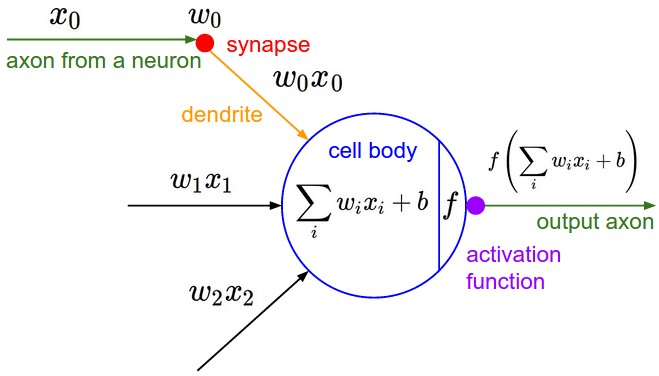
\includegraphics[width=0.6\paperwidth]{neuron_model.jpeg}}

\small source: \href{https://www.cs.utoronto.ca/~fidler/teaching/2015/slides/CSC2523/CNN-tutorial.pdf}{https://www.cs.utoronto.ca/~fidler/teaching/2015/slides/CSC2523/CNN-tutorial.pdf}

\Que{Give examples of activation functions}

\begin{itemize}
    \item Step-function $$f(x)=\begin{cases} 1, x>0 \\ 0,  x<0 \end{cases}$$
    \item Sigmoid $$f(x)=\frac{1}{1+e^{-x}}$$
    \item TanH $$ f(x)=\tanh(x)$$
    \item ReLU $$f(x)=\max(0,x)$$
    \item Maxout $$f(x) = \max(w_0x + b_0, w_1x + b_1)$$
\end{itemize}
\small source: \href{https://www.cs.utoronto.ca/~fidler/teaching/2015/slides/CSC2523/CNN-tutorial.pdf}{https://www.cs.utoronto.ca/~fidler/teaching/2015/slides/CSC2523/CNN-tutorial.pdf}

\Que{What are the strong and weak sides of sigmoid activation function}

\small source: \href{https://towardsdatascience.com/understanding-neural-networks-from-neuron-to-rnn-cnn-and-deep-learning-cd88e90e0a90}{https://towardsdatascience.com/understanding-neural-networks-from-neuron-to-rnn-cnn-and-deep-learning-cd88e90e0a90}


\Que{For image and speech recognition, what kind of neural networks are better used and why?}
\begin{itemize}
    \item CNN (Convolution Neural Networks) are used for image recognition.
    \item RNN (Recurring Neural Networks) are used for speech recognition
\end{itemize}

\small source: \href{https://www.cs.utoronto.ca/~fidler/teaching/2015/slides/CSC2523/CNN-tutorial.pdf}{https://www.cs.utoronto.ca/~fidler/teaching/2015/slides/CSC2523/CNN-tutorial.pdf}



\end{document}